\section{Background}

There are a number of models that can be used for bus arrival prediction, but there are four main models that are most widely used \cite{dynamic-gps}. They are as follows: 
\begin{itemize}
    \item \textbf{Historical average models}: Also known as simple forecasting, these models make use of historical bus arrival and travel times to predict the arrival time of buses. On its own, performance could be fairly weak, due to the unreliability of traffic conditions and other factors that vary over time. For example, Jeong and Rilett found that their historical model was outperformed by their artificial neural network model \cite{ann-prediction}.
    \item \textbf{Regression models}: These models are a form of predictive technique, which can be used to investigate the relationship between factors that affect bus arrival times (predictors) and bus arrival times (target) \cite{regression-techniques}. This technique will help to see which factors are more or less important. For example, Patnaik et al. used regression models to discover that "weather variables were not among the significant factors for estimating arrival times" \cite{apc-estimation}. 
    \item \textbf{Kalman Filtering models}: The Kalman filter is one of the optimal solutions for tracking and data prediction tasks. These models are a dynamic estimation technique that have been used fairly frequently in bus delay predictions. However, as Sun et al. found, these models are expensive to compute \cite{smart-public-transport}.
    \item \textbf{Artificial Neural Network models}: These models have been widely used in research to try to improve public transportation. They are suited towards more complex and noisy data and finding non linear relationships between dependent and independent variables \cite{dynamic-gps}. 
\end{itemize}

In this project, data that is used for the modelling is collected from TfL's publicly available APIs.

\subsection{Transport for London APIs}
\label{section:tfl-api}

Across the entire London transport system there are over 19,000 bus stops, 700 bus routes, 8,000 buses and approximately 130,000 bus arrival predictions at any point in time \cite{tfl-bus-documentation}. However, Transport for London (TfL) does not provide an API that gives exact bus arrival times and so this information has to be inferred from the Countdown API which provides estimated arrival times \cite{tfl-api}.

\subsubsection{Countdown API}

The Countdown API provides real time predicted arrival times for buses in London. The expected arrival times are updated at the Countdown source every 30 seconds, so there is some room for error in regards to the inferred arrival time of the buses. This also means that there is no point in requesting information more frequently than every 30 seconds. \\

Depending on the request, the response can be made up of 5 different array types: \texttt{Stop, Prediction, Flexible, Message} and \texttt{URA Version} arrays. The sequence of these arrays in the response is undefined except that the \texttt{URA Version} array always appears first. For the purpose of this project, the arrays that are relevant and will be returned are the \texttt{URA Version} array and the \texttt{Prediction} array. \\

An example request where Countdown was called for bus route 9 and stop code 490010357F (commonly known as \textsc{North End Road}) can be seen in Figure \ref{fig:countdown-req}. The following parameters are set: 
\begin{itemize}
    \item stop code 2: the unique national identifier of the bus stop. Not to be confused with stop code 1 which is the public code for the bus stop displayed on the bus stop flag.
    \item line name: the route number displayed on the front of the bus.
\end{itemize}

\begin{figure}[H]
\begin{center}
    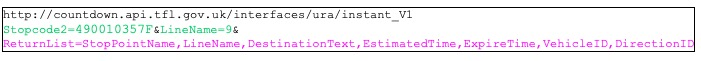
\includegraphics[keepaspectratio, width=17cm]{Images/countdown-req.jpg}
    \caption{Countdown API request}
    \label{fig:countdown-req}
\end{center}
\end{figure}

Figure \ref{fig:countdown-req} also demonstrates that users can choose what parameters Countdown should return in the response. For this project the following fields are set and returned in the \texttt{Prediction} array: 
\begin{itemize}
    \item \texttt{response type}: this is returned by default and is always 1 for the \texttt{Prediction} array.
    \item \texttt{stop name}: name of the bus stop.
    \item \texttt{line name}: the route number displayed on the front of the bus.
    \item \texttt{direction id}: 1 = outbound or 2 = inbound.
    \item \texttt{destination text}: the full length destination name of the trip the vehicle is on.
    \item \texttt{vehicle id}: the unique identifier of the vehicle.
    \item \texttt{estimated arrival time}: absolute time in UTC as per Unix epoch (in milliseconds).
    \item \texttt{expiry time}: time at which the corresponding prediction is no longer valid and should no longer be used. In this case it is the estimated arrival time + 30 seconds. 
\end{itemize}
The response also contains the timestamp that the response was processed in the \texttt{URA Version} array. \\

The Countdown API returns a JSON of the form \texttt{[[URA array],[Prediction Array]]}. An example response where Countdown was called for bus route 9 and stop code 490010357F (commonly known as \textsc{North End Road}) is seen in Table \ref{table:ura-array-stopa} and Table \ref{table:prediction-array-stopa} (the JSON information has been displayed in a table for ease of reading). Countdown was called at: Friday 15th May at 07:02:06 (time A).

\begin{table}[H]
    \centering
    \begin{tabular}{|c|c|c|}
        \hline
          Response Type & URA Version & Time that response was processed \\
        \hline
           4  & "1.0" & May 15, 2020 07:02:06.913 \\
        \hline
        \end{tabular}
    \caption{\texttt{URA Version} Array Route 9 at \textsc{North End Road} at Time A}
    \label{table:ura-array-stopa}
\end{table}

\begin{table}[H]
    \centering
    \setlength\tabcolsep{2pt}
    \begin{tabular}{|c|c|c|c|c|c|c|c|}
        \hline
          Response & Stop   &   Line & Direction & Destination & Vehicle & Estimated & Expiry \\[-3pt]
           Type & Name &    Name & ID &  Text & ID & Arrival &  Time \\
        \hline
             & "North &  &  &  &  & May 15, 2020  & May 15, 2020 \\[-3pt]
            1 & End Road" & "9" & 2 & "Aldwych" & 14510 & 07:01:57 & 07:02:27 \\
        \hline
             & "North &  &  &  &  & May 15, 2020 & May 15, 2020 \\[-3pt]
            1 & End Road" & "9" & 2 & "Aldwych" & 15448 & 07:10:02 & 07:10:32 \\
        \hline
        \end{tabular}
    \caption{\texttt{Prediction Array} Route 9 at \textsc{North End Road} at Time A}
    \label{table:prediction-array-stopa}
\end{table}

When Countdown was called to give the expected arrival time on route 9 for \textsc{North End Road}, it was also called at the same time to give the response for \textsc{Kensington Olympia Station}. Table \ref{table:prediction-array-stopb} shows the \texttt{Prediction Array} for bus route 9 and stop code 490008652A (commonly known as \textsc{Kensington Olympia Station}). Note that \textsc{Kensington Olympia Station} is the immediate station after \textsc{North End Road} in the 9 route to "Aldwych". Comparing Table \ref{table:prediction-array-stopa} and Table \ref{table:prediction-array-stopb}, it can be seen that the two same vehicles appear in both responses. This response can be interpreted visually as in Figure \ref{fig:countdown-response-timeA}.

\begin{table}[H]
    \centering
    \setlength\tabcolsep{2pt}
    \begin{tabular}{|c|c|c|c|c|c|c|c|}
        \hline
          Response & Stop   &   Line & Direction & Destination & Vehicle & Estimated & Expiry \\[-3pt]
            Type & Name &    Name & ID &  Text & ID & Arrival &  Time \\
        \hline
             & "Kensington &  &  &  &  & May 15, 2020 & May 15, 2020 \\[-3pt]
            1 & Olympia Station" & "9" & 2 & "Aldwych" & 14510 & 07:02:49 & 07:03:19 \\
        \hline
             & "Kensington &  &  &  &  & May 15, 2020 & May 15, 2020 \\[-3pt]
            1 & Olympia Station" & "9" & 2 & "Aldwych" & 15448 & 07:10:54 & 07:11:24 \\
        \hline
        \end{tabular}
    \caption{\texttt{Prediction Array} Route 9 at \textsc{Kensington Olympia Station} at Time A}
    \label{table:prediction-array-stopb}
\end{table}

When Countdown is called again at Friday 15th May at 07:02:43 (time B) for both \textsc{North End Road} and \textsc{Kensington Olympia Station}, the new response can be seen visually interpreted in Figure \ref{fig:countdown-response-timeB}. It can be seen that bus 14510 has now arrived at and passed \textsc{North End Road} and is on its way to \textsc{Kensington Olympia Station}. This is indicated by the JSON response shown in Table \ref{table:prediction-array-stopa-updated} where bus 14510 is no longer returned in the \texttt{Prediction Array} for Route 9 at \textsc{North End Road}.

\begin{table}[H]
    \centering
    \setlength\tabcolsep{2pt}
    \begin{tabular}{|c|c|c|c|c|c|c|c|}
        \hline
          Response & Stop   &   Line & Direction & Destination & Vehicle & Estimated & Expiry \\[-3pt]
           Type & Name &    Name & ID &  Text & ID & Arrival &  Time \\
        \hline
             & "North &  &  &  &  & May 15, 2020 & May 15, 2020 \\[-3pt]
            1 & End Road" & "9" & 2 & "Aldwych" & 15448 & 07:10:02 & 07:10:32 \\
        \hline
        \end{tabular}
    \caption{\texttt{Prediction Array} Route 9 at \textsc{North End Road} at Time B}
    \label{table:prediction-array-stopa-updated}
\end{table}

\begin{figure}[H]
\begin{center}
    \includegraphics[keepaspectratio, width=14cm]{Images/Countdown-response-timeA.png}
    \caption{Countdown API response at time A}
    \label{fig:countdown-response-timeA}
\end{center}
\end{figure}

\begin{figure}[H]
\begin{center}
    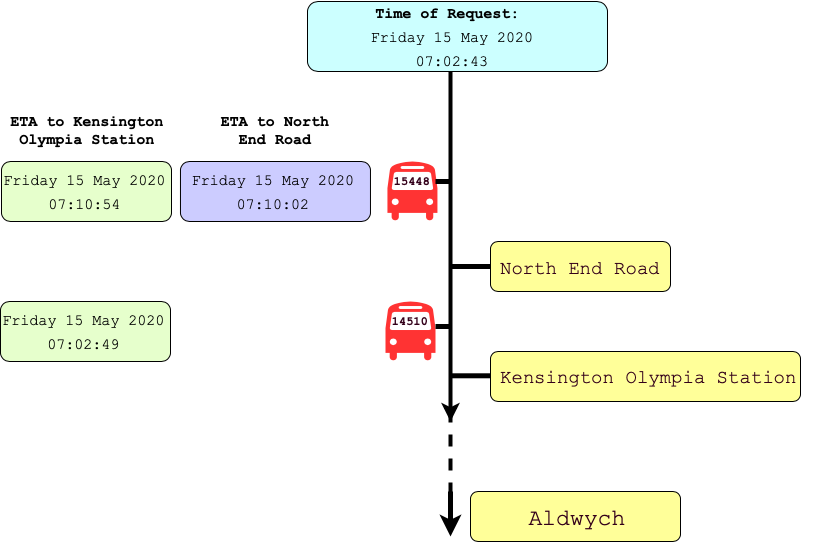
\includegraphics[keepaspectratio, width=14cm]{Images/Countdown-response-timeB.png}
    \caption{Countdown API response at time B}
    \label{fig:countdown-response-timeB}
\end{center}
\end{figure}

\subsubsection{Stoppoints API}

This API is called to give information on all bus stops for a particular route. A request takes the form:

\begin{center}
\texttt{https://api.tfl.gov.uk/line/bus\_route\_id/stoppoints}.
\end{center}

The response returns an array of stops. For each stop, information includes bus stop name, bus stop letter, all lines/routes serving that stop, facilities at the stop, including toilets, WiFi, phone number etc. and latitude and longitude. However, this API returns more stop IDs than there actually are stops on a route. When put as parameters into the Countdown API call, some of the stops return estimated arrival times as expected, whereas others return HTTP errors. A possible explanation for this could be differences in routing or bus stop additions/deletions over the years. Therefore, it is useful to verify which stop ids are valid and which are invalid. 

\subsubsection{Stoppoints Sequence API}

This API is called to give the list of stops in the order that they are visited for a particular route. It can be called for both bus and underground routes. A request takes the form: 

\begin{center}
    \texttt{https://api.tfl.gov.uk/Line/bus\_route\_id/Route/Sequence/outbound}
\end{center}

For each of the stops returned in the list, the response also gives the interchanges with other lines and modes. The response also returns the latitude and longitude showing the path of the route so it can be plotted on a map.

\subsection{Historical Average Models}
\label{section:historical-avg-models-research}

Historical average models or forecasting models have some of the simplest algorithms. This tends to lead to shorter computation times, which in this case, could be very useful because of the sheer volume of data across London's bus network. However, unless the bus journey times are fairly constant in history, it is easy for the model performance to be weaker than other types of models. 

\subsubsection{Forecasting}
Forecasting is an important aid to effective and efficient planning. Statistical forecasting typically refers to the use of statistics on historical data to project what could happen in the future \cite{what-is-forecasting}. The effectiveness of forecasting as a method depends on several factors including: how well we understand the factors that contribute to an event, how much data is available and whether the forecasts can affect the thing we are trying to forecast \cite{forecasting-book}. A good forecast should capture the genuine patterns and relationships which exist in the historical data, but do not replicate past events that will not occur again. In the case of historical bus data, the data collected will be gathered at regular intervals over time, and therefore, can be seen as time series data. In this way, quantitative forecasting can be applied because it is reasonable to assume that some aspects of the past patterns will continue into the future.

\subsubsection{Methods}

When forecasting time series data, the aim is to estimate how the sequence of observations will continue into the future. The simplest time series forecasting methods only use information on the variable to be forecast without attempting to discover the factors that could affect its behaviour. Therefore, these methods will extrapolate trends and seasonal patterns, but will ignore other information. For example, when forecasting bus arrival times, we would look at historical information on bus delays, but would ignore factors such as traffic conditions or weather conditions. \\

Some of the most common simple forecasting methods are listed below \cite{forecasting-book}:

\begin{itemize}
    \item \textbf{Mean Method}: All the future forecast values are equal to the average of the historical data. This method is optimal when data has a fairly steady value and does not change much over time.
    \item \textbf{Naive Method}: All the future forecast values are equal to the value of the last observation. This method is optimal when data follows a random walk.
    \item \textbf{Seasonal Naive Method}: Each forecast value is set to be equal to the last observed value from the same season of the year, for example from the same month of the previous year or the same quarter of the previous year. This method tends to perform better than a simple naive method, especially when the historical data has a clear seasonal trend. 
    \item \textbf{Drift Method}: This method is a variation of the naive method. The forecast values increase or decrease over time and the amount of change over time is called the drift. This drift is set to be the average change seen in the historical data. This method is equivalent to drawing a straight line between the first and last observations and extrapolating it into the future. 
\end{itemize}

Figure \ref{fig:forecasting} shows what the \textit{mean}, \textit{naive} and \textit{seasonal naive} methods look like when applied to quarterly beer production data. It can be seen that both the \textit{mean} and \textit{naive} methods result in flat line forecasts, and therefore, would not be particularly suitable for bus arrival predictions because research has shown that for different time periods, the trends in journey times vary \cite{dynamic-gps}, \cite{ann-prediction}, \cite{smart-public-transport}. However, a slight variation on the mean and naive method that essentially combines the two methods, where the model takes the average of the last two or three bus travel times for each forecast, is much more likely to provide a better estimate. This is because this method will use historical results that should theoretically be in the same time period as the current time to be forecast. This method will also avoid going too far into the past and using data that may not be relevant. Figure \ref{fig:forecasting} also shows that the \textit{seasonal naive} method results in an oscillating prediction. Since there is reason to believe that historical data on bus delay times show an up and down trend, the seasonal naive method could also be an equally suitable model to use.

\begin{figure}[H]
\begin{center}
    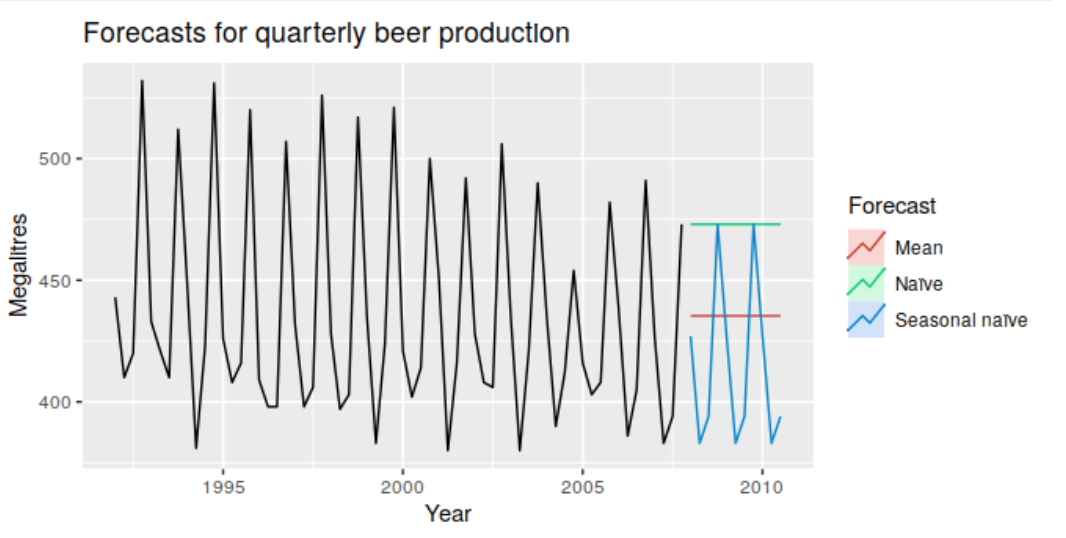
\includegraphics[width=\textwidth]{Images/forecasting-beer-prod.png}
    \caption{Example of the mean, naive and seasonal naive methods, original image from \cite{forecasting-book}}
    \label{fig:forecasting}
\end{center}
\end{figure}

\subsubsection{Measuring Success}

A forecast may be greater than or less than the actual value. The difference between this predicted value and the actual value is called the forecast error. Equation \ref{eq:forecast-error} shows the forecast error for an individual forecast \cite{forecasting-performance-measures}.

\begin{equation}
\label{eq:forecast-error}
    \mathrm{FE}_t = A_t - F_t
\end{equation}

\noindent where FE$_t$ is the forecast error, $A_t$ is the actual value and $F_t$ is the forecasted value. \\

Measures to evaluate the performance of a forecasting method can be classified into those that look at direction and those that look at size of the error. The bias (Equation \ref{eq:forecast-bias}) is the most popular measure for evaluating the direction of the error, i.e. whether the predictions are over or under the actual values. The closer the bias is to zero, the better the model. If the bias is negative, this implies that the actual values are on average, smaller than the predicted value. Therefore, the forecasting model overestimates the actual values. Let $n$ be the number of samples, then:

\begin{equation}
\label{eq:forecast-bias}
    Bias = \frac{\sum(A_t-F_t)}{n}
\end{equation}

The size of the error could mean the amount of the error or the dispersion of the error or the relative magnitude of the error. One of the most popular measures of the size of the error is the mean squared error (MSE). The MSE (Equation \ref{eq:forecast-mse}) is the average of the sum of squares of the forecast errors and measures the amount of dispersion in the error. The smaller the value, the better.

\begin{equation}
\label{eq:forecast-mse}
    MSE = \frac{\sum(A_t-F_t)^2}{n}
\end{equation}

Another common measure is the root mean squared error (RMSE), which is, as its name suggests, the square root of the MSE. The RMSE measures how spread out the residuals are, where the residuals are how far away from the regression line the data points are. More intuitively, the RMSE describes how concentrated the data is around the line of best fit. However, neither the MSE nor the RMSE take into account the magnitude of the actual values. \\

A measure of success that does attempt to take into account the effect of the magnitude of the actual values is the mean absolute error (MAE). The MAE (Equation \ref{eq:forecast-mae}) is the average of the absolute values of the errors. As with the RMSE and MSE, the smaller the value, the better.

\begin{equation}
\label{eq:forecast-mae}
    MAE = \frac{\sum|A_t-F_t|}{n}
\end{equation}

The RMSE is bounded by the MAE:

\begin{itemize}
    \item MAE $\leq$ RMSE: The RMSE will always be larger or equal to the MAE. If all of the errors have the same magnitude, then the two values are equal.
    \item RMSE $\leq$ (MAE * $\sqrt{n}$): The difference between the RMSE and the MAE is greatest when all of the prediction error comes from a single test sample. This implies that as the sampel size increases, the RMSE tends to become increasingly larger than the MAE. 
\end{itemize}

\subsection{Regression Models}
\label{section:regression-models-research}

Regression is a form of statistical modelling that investigates the relationship between a dependent (target) and independent (predictor) variable \cite{regression-techniques}. When performing statistical modelling, we observe some data $y$, known as the dependent variable, and interpret each data point as a realisation of some random variable $Y$, following some probability distribution. A statistical model is a specification of the distribution of $Y$ up to an unknown parameter $\theta$. Often $y = (y_1, y_2, ..., y_n) \in \mathbb{R} ^ n$ is a vector and $Y = (Y_1, ..., Y_n)$ is a random vector. The distribution of $Y_1, ..., Y_n$ may depend on (non random or deterministic) quantities $x_1, ..., x_n$ known as covariates or predictors. \\

Regression models are suitable when the variable that is trying to be predicted relies on a number of different independent factors. This is a very important point to ensure since non-independence is a reason for sub-optimal predictions in linear models. Since it is hypothesised that the journey time of a bus relies on many things such as weather conditions, time of day, traffic conditions and so on, this makes regression models a good choice to implement. Regression models also help to see which of these independent variables are statistically significant, and so can provide insight into which of the factors that are being considered are worth being explored further. However, the viability of regression models is limited by the hypothesis that many of the factors affecting bus journey times are in fact correlated to one another and not independent after all. 

\subsubsection{Linear Regression}

In the simplest case, the regression model allows for a linear relationship between the observable variable $Y$ and a single predictor variable $x$ (Equation \ref{eq:lin-reg}): 

\begin{equation}
    Y_t = \beta_1 + x_i\beta_2 + \epsilon_t, t = 1, ..., n
    \label{eq:lin-reg}
\end{equation}

where $Y_t$ is the outcome or observable random variable, $x_t$ is the covariate constant, $\beta_0$ and $\beta_1$ denote the intercept and slope of the line respectively and $\epsilon_t$ are iid (independent and identically distributed) errors. $E(\epsilon_t) = 0$, $Var(\epsilon_t) = \sigma^2$ for $t = 1,...n$. $\sigma^2 > 0$ is also unknown. The errors are not observable and can be thought of as the deviation from the underlying straight line model, capturing anything that may affect $Y_t$ other than $x_t$ \cite{forecasting-book}. Figure \ref{fig:lin-reg} visualises the linear relationship as defined in Equation \ref{eq:lin-reg}.

\begin{figure}[H]
\begin{center}
    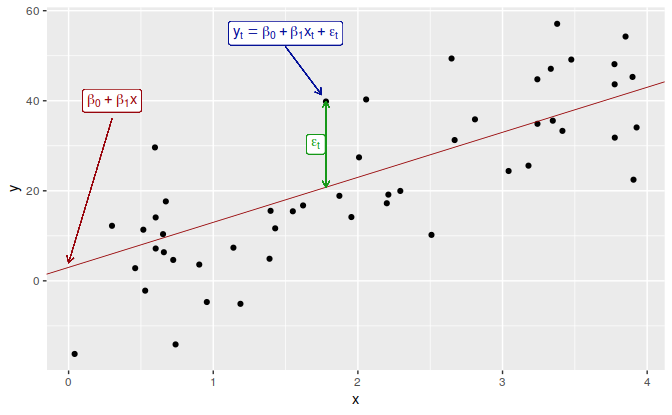
\includegraphics[width=\textwidth]{Images/linear-regression.png}
    \caption{Linear Regression, original image from \cite{forecasting-book}}
    \label{fig:lin-reg}
\end{center}
\end{figure}

\subsubsection{Multiple Linear Regression}

When there are two or more predictor variables, the model is called a multiple regression model. The general formulation in a linear model is shown in Equation \ref{eq:multi-regression}:

\begin{equation}
    Y = \mathbf{X}\beta + \epsilon
    \label{eq:multi-regression}
\end{equation}

where $Y$ is an n-dimensional random vector (observable), $\mathbf{X} \in \mathbb{R} ^{n \times p}$ is a known matrix (often called the `design matrix'), $\beta \in \mathbb{R}^p$ is an unknown parameter and $\epsilon$ is an n-variate random vector (not observable) with $E(\epsilon) = \mathbf{0}$. The $\beta$ coefficients essentially measure the effect of each predictor after taking into account the effects of all the other predictors in the model. \\

When we use a linear or multiple regression model, we make the following assumptions.

\begin{itemize}
    \item The model is a reasonable approximation to reality, that is, the relationship between the forecast variable and the predictor variable satisfies this linear equation.
    \item We make the following assumptions about the errors:
    \begin{itemize}
        \item they have a mean of zero; otherwise the predictions will be systematically biased.
        \item they are not autocorrelated; otherwise the predictions will be inefficient.
        \item they are unrelated to the predictor variables; otherwise there would be more information that should be included as a predictor variable.
    \end{itemize}
    \item Each predictor $x$ is not a random variable.
\end{itemize}

\subsubsection{Pearson Correlation Coefficient}

The Pearson correlation coefficient, commonly written simply as $\rho$ is the measure of the linear relationship between two variables \cite{correlation-coeff-journal}, \cite{correlation-coeff}. It is calculated as the covariance of the two variables divided by the product of the standard deviation of each data sample. In other words, it is the normalization of the covariance between the two variables. Given a pair of variables $(X, Y)$, the Pearson correlation coefficient follows Equation \ref{eq:correlation-coeff}:

\begin{equation}
\label{eq:correlation-coeff}
    \rho_{X,Y} = \frac{cov(X,Y)}{\sigma_X\sigma_Y}
\end{equation}

where $cov$ is the covariance, $\sigma_X$ is the standard deviation of $X$ and $\sigma_Y$ is the standard deviation of $Y$. \\

The coefficient is bounded between $-1$ and $1$, where values near $0$ indicate no correlation. Positive values indicate a positive correlation, where the larger $X$ gets, the larger $Y$ also gets. Negative values indicate a negative correlation, where as $X$ increases, $Y$ decreases.

\subsubsection{Measuring Success}

The standard error is equal to the standard deviation, which would be obtained from repeatedly estimating the $\beta$ coefficients on similar data sets. This gives a measure of the uncertainty in the estimated $\beta$ coefficient. \\

The p-value is the probability of the estimated $\beta$ coefficient being as large as it is if there was no real relationship between the forecast variable and the corresponding predictor. This is particularly useful when studying the effect of each predictor, and can be used as another way of seeing which parameter to use in the models and which to discard. \\ 

A common way to summarise how well a regression model fits the data is via the coefficient of determination (Equation \ref{eq:r-squared}:

\begin{equation}
    R^2 = \frac{\sum(\hat y_t - \bar y)^2}{\sum(y_t - \bar y)^2}
    \label{eq:r-squared}
\end{equation}

where the summations are over all the observations, $\hat y_t$ are the predicted values, $y_t$ are the observed values and $R^2$ is bounded between 0 and 1. Although this is a way of measuring `goodness-of-fit', validating the performance of a model against a test set is much better than measuring the $R^2$ value on the training data \cite{forecasting-book}. \\

The differences between the observed $y$ values and the corresponding fitted $\hat y$ values are known as residuals. To detect problems with a model, we can plot standardised residuals against some each of the predictor variables. We expect the residuals to be randomly scattered without showing any systematic pattern because a pattern would indicate a nonlinear relationship between the variables. If the model is correct then the resulting plot should just show `noise' with no distinct patterns. \\

As with the historical models, the mean absolute error (MAE) and the root mean squared error (RMSE) can also be used as measures of success.

\subsection{Kalman Filtering Models}
\label{section:kalman-models-research}

Kalman filtering is a dynamic two-step algorithm that uses measurements observed over time to estimate some unknown variables \cite{kalman-korean}. The first part is the prediction process and the second part is the measurement process. The two processes are modelled by groups of equations in the state space model. Kalman filter models generally provide good predictions because they are able to optimally estimate the system's error covariance and recursively use the prediction to improve the system measurements \cite{kalman-malay}. In this case, the journey time of a future bus would be predicted based on the system's state in past time steps. Kalman Models also have great capabilities of filtering out noise.  \\

Kalman filter models would be suitable for the task of estimating bus arrival times because unstable traffic conditions can be accommodated by their time dependent parameters \cite{dynamic-gps}. Furthermore, Kalman filter models are able to make predictions based purely on journey times, without the need for other traffic conditions. However, Kalman filter models struggle to handle abrupt changes between consecutive travel times. So, if there was a significant difference in travel times between the morning peak and late morning hours, the model is unable to filter the noise smoothly. 

\subsection{Artificial Neural Network Models}
\label{section:ml-models-research}

(Feed-forward) Artificial Neural Networks (ANNs) are a type of machine learning inspired by real world biological neurons. \\

ANNs have the ability to solve complex non-linear relationships and can capture subtle relationships between the data, even if the underlying relationships are unknown \cite{dynamic-gps}. Therefore, ANNs are a popular choice for bus prediction models because it can learn the non-linear correlations between bus travel times. If the ANN has enough neurons in the hidden layers, then it is very capable of arbitrary input-output matching \cite{intelligent-transport-systems}. However, this also implies that ANNs have a high potential for over-fitting and therefore, could struggle to generalise to data not given in the training process. This over-fitting is also what makes ANNs so resource intensive. Furthermore, the back propagation algorithm, which is the most used algorithm for transportation problems, has a long learning process. \\

ANNs are also harder to interpret compared to historical models and regression models. For example, the coefficients gotten from the regression model describe the relative importance of each of the factors. However, the weights and biases gotten after training a neural network model are not as easy to understand intuitively. 

\subsubsection{Perceptrons}

An ANN has a collection of nodes called artificial neurons, the most common type of which is called a perceptron \cite{methods-for-ds-slides}, \cite{neural-networks-book}. A perceptron takes $m + 1$ inputs $x_{i\in{0,...,m}}$ with $m + 1$ weights $w_{i\in{0,...,m}}$ and produces a single binary output $y$. Weights are real numbers expressing the importance of the respective inputs to the output. So a perceptron's output, 0 or 1, is determined by whether the weighted sum is less than or greater than some threshold value (Equation \ref{eq:perceptron}).

\begin{equation}
    output = 
    \begin{cases} 
        0 \textrm{ if } \sum_jw_jx_j \leqslant \textrm{threshold} \\
        1 \textrm{ if } \sum_jw_jx_j > \textrm{threshold}
    \end{cases}
    \label{eq:perceptron}
\end{equation}

By varying the weights and the threshold, we can get different models of decision making. We set the bias of a perceptron to be $w_0$ and set $x_0 = 1$. The bias is a measure of how easy it is to get the perceptron to output a 1. The perceptron can be `activated' using a non linear activation function $g$, allowing us to approximate arbitrarily complex function. \\

There are a number of different activation functions, with some common ones including the \textit{Sigmoid} function: $ \sigma(x) = \frac{1}{1 + e^{-x}} $ and the \textit{ReLU} function: $ max(0, x) $. Figure \ref{fig:perceptron} shows a single perceptron with 3 input neurons ($x_0$ = 1 and $w_0$ is the bias) and output $\mathbf{\hat y}$.

\begin{figure}[H]
\begin{center}
    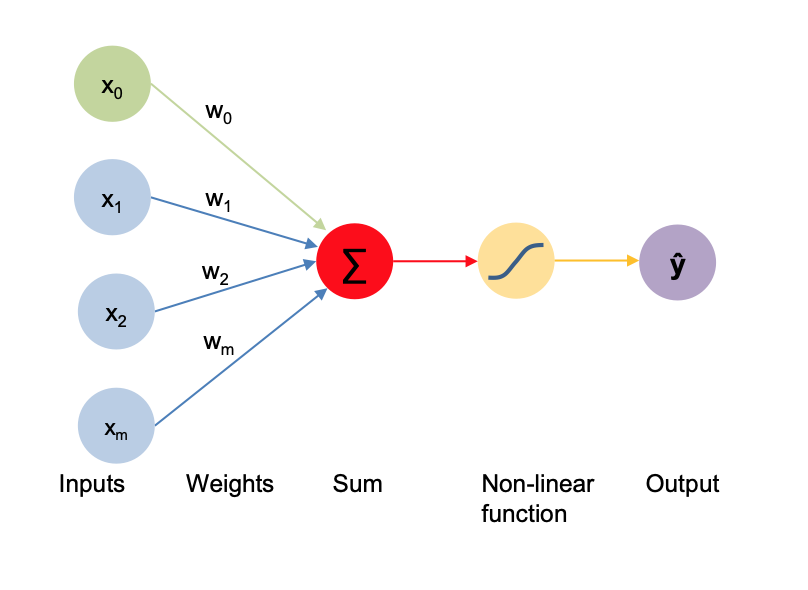
\includegraphics[scale=0.8]{Images/perceptron-forward-prop.png}
    \caption{The Perceptron: forward propagation, original image from \cite{methods-for-ds-slides}}
    \label{fig:perceptron}
\end{center}
\end{figure}

\subsubsection{Architecture}

ANNs consists of stacking neurons into layers, with different layers performing transformations on their inputs. These models are called feed-forward because information flows from input $x$ to output $y$ without any feedback connections in which outputs of the model are fed back into itself, i.e. information always travels forward \cite{deep-learning-book}. Figure \ref{fig:nn-architecture} shows a fully connected neural network with a single layer. The leftmost layer is called the input layer, the rightmost layer is called the output layer and the middle layers are called hidden layers. Neural networks with multiple hidden layers are sometimes called multi-layer perceptrons.

\begin{figure}[H]
\begin{center}
    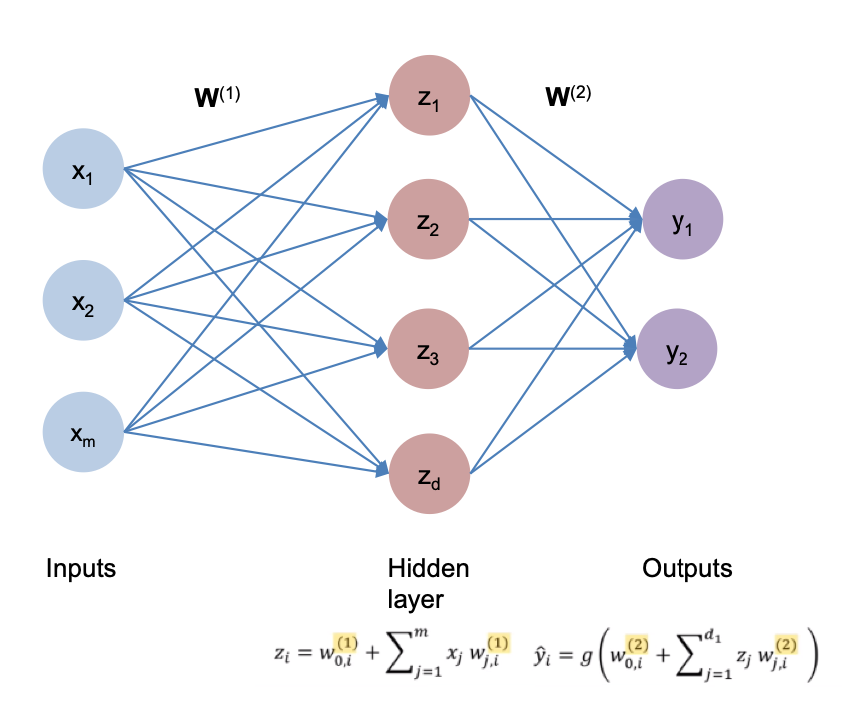
\includegraphics[scale=0.8]{Images/single-layer-nn.png}
    \caption{Fully connected single layer neural network, original image from \cite{methods-for-ds-slides}}
    \label{fig:nn-architecture}
\end{center}
\end{figure}

\subsubsection{Back Propagation}

The desired output from the output layer neurons is known. During the training process, the network uses the given examples to adjust the weights between the neurons to produce the known output. The error in the output is propagated back through the layers to help in the weight adjustment decisions \cite{ann-prediction}.

\subsubsection{Regularization and Overfitting}

Regularization is implemented to constrain the optimization problem, ensuring that our model can generalize to unseen data and not overfit. One method of regularization is to implement dropouts. This randomly sets some of the neurons to 0, typically 50\% of neurons in each layer, preventing reliance on a single node \cite{methods-for-ds-slides}. Another regularization method is early stopping. Here, we stop training the model as soon as the desired accuracy is reached or as soon as overfitting is detected. Generally, the variance or error increases in overfitted models. 

\subsection{Numerical Interpolation and Approximation}

Numerical interpolation is the process of attempting to fit a function to given data points \cite{intro-to-numerical-analysis-atkinson}. In interpolation, the data is fitted exactly, while in approximation this is not the case. Interpolation is not appropriate when the data points are likely to have experimental errors (for example errors that occur when the data is being collected). Therefore, since this project requires the bus data to be collected manually and thus there is room for human error, this is an argument against the use of an interpolation model. On the other hand, combining regression analysis with interpolation allows models to take into consideration the actual, fluctuating travel conditions and thus provide predictions with more flexibility \cite{aviation-regression-interpolation}.

\subsubsection{Linear Interpolation}

Linear interpolation models search for a straight line that passes through the given end points $x_A$ and $x_B$ as shown in Equation \ref{eq:linear-interpolation} \cite{interpolation-in-time-series}.

\begin{equation}
    \label{eq:linear-interpolation}
    X_i = (1-\alpha)x_B + \alpha x_A
\end{equation}

where $\alpha$ is the interpolation factor, varying from 0 to 1. The interpolated data is bound between $x_A$ and $x_B$.

\subsubsection{Polynomial Interpolation}

Polynomial interpolation models search for a polynomial that fits exactly with the given information about a real valued function $f$ of a single real variable $x$ \cite{intro-to-numerical-analysis-suli}, assuming that there is always a unique polynomial of degree at most $n-1$ passing through $n$ data points. The corresponding polynomial is called the Lagrange interpolation polynomial. If $f$ is differentiable, the corresponding polynomial, called the Hermite interpolation polynomial, may include values of the derivative of $f$ at some finite set of points. \\

If the function values $f(x)$ are known for all $x$ in a closed interval of the real line, then the aim of polynomial interpolation is to approximate the function $f$ by a polynomial over this interval. However, if the function values $f(x)$ are only known for a finite set of points $x_0, ..., x_n$, then the aim of polynomial interpolation is to construct the unknown function $f$ by seeking a polynomial $p_n$. Where $p_n$ passes through the points with co-ordinates $(x_i, f(x_i)$ for $i = 0, ..., n$ on the $(x, y)$ plane \cite{intro-to-numerical-analysis-suli}. \\

However, fitting a single polynomial to a large number of data points tends to lead to overfitting because the function oscillates between the data points \cite{intro-to-numerical-analysis-atkinson}. Piece-wise interpolation attempts to solve this issue. 

\subsubsection{Piecewise Interpolation}

Piecewise interpolation models attempt to fit a number of different low-degree polynomials to a large number of data points \cite{intro-to-numerical-analysis-atkinson}. This eliminates excessive oscillations and non-convergence.\\

Subdivide $[a, b]$ into $J$ equal subintervals $[x_{j-1}, x_j]$ for $j = 1, ..., J$ of length $h$. Let $h = \frac{b-a}{j}$ then 

\begin{equation}
    x_j = a + jh, j = 0, ..., J
\end{equation}

\begin{figure}[H]
\begin{center}
    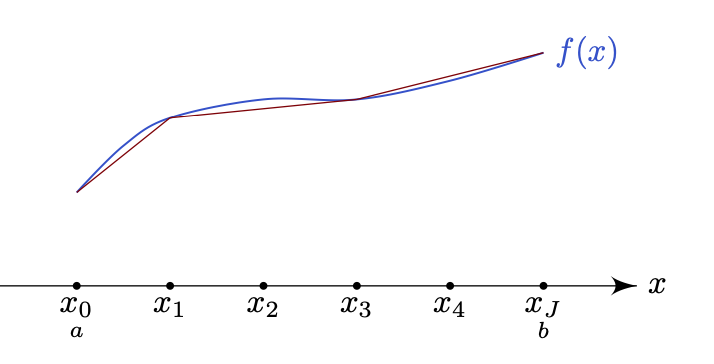
\includegraphics[width=10cm]{Images/piecewise-polynomial-interpolation.png}
    \caption{Piecewise polynomial interpolation, original image from \cite{m2aa3-notes}}
    \label{fig:piecewise-polynomial-interpolation}
\end{center}
\end{figure}

On each subinterval $[x_{j-1}, x_j]$ for $j = 1,...,J$ linear interpolation is performed. \\

A problem with piecewise interpolation is that the graphs can have corners at which points the derivative is discontinuous. In other words, the interpolation is not as smooth.

\subsubsection{Piecewise Polynomial Approximation}

Divide the interval $[a,b]$ into a number of subintervals and for each subinterval, attempt to approximate it by a polynomial of low degree. These piece-wise polynomial approximations are called \textit{splines} and the endpoints of the subintervals are called \cite{intro-to-numerical-analysis-suli}. A spline of degree $n$, $n \geq 1$ is a function which is a polynomial of degree $n$ or less in each subinterval. Splines have continuous derivatives of order up to $k$ for $0 \leq k < n$. If the derivative of order n is required to be continuous everywhere, then the spline is just a single polynomial. \\

A particular example is a cubic spline. Consider the set $S$ of all functions $s \in C^2[a,b]$ such that Equation \ref{eq:cubic-spline-a} and Equation \ref{eq:cubic-spline-b} are true.

\begin{equation}
\label{eq:cubic-spline-a}
    s(x_j) = f(x_j),\ j = 0,...,J
\end{equation}

\begin{equation}
\label{eq:cubic-spline-b}
    s \textrm{ is a cubic on } [x_{j-1}, x_j],\ j=1,...,J
\end{equation}

Any element of $S$ is referred to as an interpolating cubic spline. There is more than 1 interpolating cubic spline that satisfies the conditions. Indeed there are $4J$  coefficients of cubic polynomials and only $J+1$ interpolating conditions and $3(J-1)$ continuity conditions. Since $s$ belongs to $C^2[a, b]$ this means that $s$, $s'$ and $s''$ are continuous at the internal knots $x_1, ..., x_{J-1}$ \cite{intro-to-numerical-analysis-suli}. \\

A special case of the cubic spline is the natural cubic spline, which must also satisfy Equation \ref{eq:cubic-spline-c}. This condition means that the piece-wise cubic polynomial is twice continuously differentiable and has less tendency to osciltate between data points. The natural cubic spline is linear at the boundary subintervals, resulting in less boundary bias.

\begin{equation}
    \label{eq:cubic-spline-c}
     s''(x_0) = s''(x_j) = 0
\end{equation}

\subsubsection{Measuring Success}

As with the historical models, the mean absolute error (MAE) and the root mean squared error (RMSE) can also be used as measures of success.

\subsection{Exploratory Data Analysis}

It is important to explore the dataset being used for a number of reasons including: extracting important variables, identifying outliers or human error and understanding the relationships (or lack of) between variables \cite{significance-of-eda}. \\

Descriptive statistic methods include looking at the mean, median, variance, interquartile range and skewness. Visualisation methods include creating histograms, density graphs and scatter plots. More complex methods include dimensionality reduction and cluster analysis. 

\subsubsection{Outliers}

An outlier is an observation that is distant from all the other data points in a dataset. If an observation has been identified as a likely outlier, it is important to try and analyse why it is the case, as outliers can arise from incorrect data collection or can be an indication of the underlying model being unsuitable \cite{forecasting-book}. Since the data used for the bus journey modelling is manually collected, there is room for human error and therefore, it is important to ensure the outliers are detected and removed accordingly. \\

Observations that have a large influence on the estimated coefficients of a regression model are called influential observations. They depend on the residual (the vertical distance) and the leverage (the horizontal distance). Figure \ref{fig:outlier} is an example showing how an outlier can affect predictions. The red line is the regression line fitted to the data including the outliers, the black line is the regression line fitted to the data without the outlier. It can be seen that the gradient of the 2 lines are not the same and therefore, the models would give differing predictions.  

\begin{figure}[H]
\begin{center}
    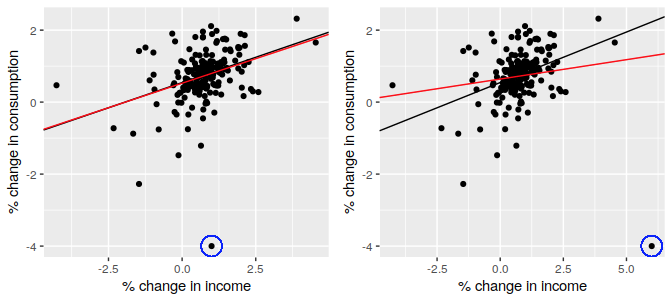
\includegraphics[width=11cm]{Images/outlier-analysis.png}
    \caption{Example showing how an outlier can affect predictions, original image from \cite{forecasting-book}}
    \label{fig:outlier}
\end{center}
\end{figure}

Data points that fall outside 1.5 times of the interquartile range above the third quartile or below the first quartile can be classed as outliers. It is also possible to identify outliers using the z-score. The z-score is the signed number of standard deviations by which the value of an observation is above the mean value of what is being observed (Equation \ref{eq:z-score}) \cite{engineering-stats-handbook}. 

\begin{equation}
    \label{eq:z-score}
    Z Score = \frac{Observation - Mean}{Standard Deviation}
\end{equation}

The calculation rescales and centers the data and looks for data points which are too far from zero. Convention is that data points that give a z-score of greater than 3 or -3 are classed as outliers. 

\clearpage
